% this file is called up by thesis.tex
% content in this file will be fed into the main document

%: ----------------------- name of chapter  -------------------------
\chapter{Phương pháp giải quyết} % top level followed by section, subsection


%: ----------------------- paths to graphics ------------------------

% change according to folder and file names
\ifpdf
    \graphicspath{{3/figures/PNG/}{3/figures/PDF/}{3/figures/}}
\else
    \graphicspath{{3/figures/EPS/}{3/figures/}}
\fi

%: ----------------------- contents from here ------------------------


\noindent Chương này chúng tôi sẽ trình bày về hệ thống theo dõi tin tức trực tuyến có tên $\mathcal{N}$\texttt{ewSOMoni}
\footnote{[nju: 's$\Lambda$m m$\Lambda$ni]} \footnote{$\mathcal{N}$\texttt{ew} \overbrace{S}^{\mbox{Smartness}} \underbrace{O}_{\mbox{Orientation}} \overbrace{M}^{\mbox{Magnitude}}oni \hspace{0.2in}   \mbox{viết tắt của \texttt{News Online Monitoring}}} cùng  phương pháp lai giữa luật và học máy Maximum Entropy trong pha trích xuất sự kiện của hệ thống vừa được nhắc tới. %Trước tiên, mô hình đề xuất và diễn giải chi tiết hệ thống được thể hiện ở phần %\ref{system} ngay dưới đây. Sau đó, phương pháp lai trích xuất sự kiện được nói %tới  ở phần \ref{method} (trang \pageref{method}).
Trước tiên, phương pháp lai giữa luật ngữ nghĩa và học máy Maximum Entropy được thể hiện ngay dưới đây. Sau đó, mô hình đề xuất và diễn giải chi tiết của hệ thống $\mathcal{N}$\texttt{ewSOMoni} được xem xét ở phần \ref{system}.



\section{Kết hợp luật ngữ nghĩa  và Maximum Entropy trong trích xuất sự kiện}
\label{method}


\section{Hệ thống theo dõi tin tức trực tuyến  $\mathcal{N}$\texttt{ewSOMoni}}
\label{system}
%\figuremacro{largepotato}{Mô hình hệ thống}{ok}}
%\figuremacro{system}{Mô hình hệ thống}}
\noindent Công trình nghiên cứu này chúng tôi đã xây dựng một hệ thống theo dõi tin tức trực tuyến. Nhiệm vụ chính của hệ thống là quan sát tức mới được đưa lên các nguồn cung cấp tin tức (phụ lục \ref{website}, trang \pageref{website}), phân loại và nhận dạng  sự kiện thuộc ba lĩnh vực: \textsc{Tai nạn giao thông}, \textsc{Hình sự}, \textsc{Cháy nổ}. Cuối cùng là trực quan hóa trên bản đồ cho người dùng dễ dàng theo dõi, cập nhật. \\
\noindent Mô hình của hệ thống được thể hiện rõ ở hình \ref{fig:system}. Hệ thống $\mathcal{N}$\texttt{ewSOMoni} có năm  phần chính:
\begin{itemize}
  \item \textbf{Kho dữ liệu} cơ sở dữ không ràng buộc, hướng tài liệu (MongoDB), lưu trữ lượng  lớn dữ liệu tin tức

\item \textbf{Thu thập dữ liệu} thu thập dữ liệu tự động và tiền xử lý dữ liệu
  \item \textbf{Phân loại sự kiện} đưa  tin tức thu thập được vào bốn dạng: \textsc{Tai nạn giao thông}, \textsc{Hình sự}, \textsc{Cháy nổ}, \textsc{Còn lại}.


  \item \textbf{Trích xuất sự kiện} thực hiện các bước cần thiết để trích xuất sự kiện
  \item \textbf{Trực quan hóa dữ liệu} có nhiệm vụ tương tác với cơ sở dữ liệu để hiển thị thông tin cho người dùng
 \end{itemize}

\noindent Mỗi thành phần của hệ thống sẽ được diễn giải chi tiết dưới đây.

\subsection{Kho dữ liệu}
\label{db}
\noindent Hệ thống phải xử lý dữ liệu lớn nên cần lựa chọn kiểu lưu trữ cũng như thiết kế cơ sở dữ liệu phù hợp. Riêng chỉ lượng dữ liệu thu thập ngoại tuyến gồm 3.842.137 tin tức điện tử phục vụ cho quá trình sinh luật và học mô hình phân lớp ban đầu đã có dung lượng gần 60GB. Hơn nữa, hệ thống chạy trực tuyến mỗi ngày nhận khoảng 1500 bài báo điện tử. Do vậy, cần thiết một hệ cơ sở dữ liệu có khả năng truy xuất dữ liệu nhanh cũng như có khả năng mở rộng về sau. Qua khảo sát, nhóm nghiên cứu nhận thấy các hệ cơ sở dữ liệu không quan hệ (NoSQL) phù hợp với tiêu chí đề ra. NoSQL không tồn tại các ràng buộc giữa các bảng lưu trữ. Điều này giúp cho tốc độ truy vấn tốt hơn hẳn so với các hệ cơ sở dữ liệu quan hệ truyền thống. Thứ nữa, NoSQL là hệ cơ sở dữ liệu phân tán, có thể mở rộng theo chiều ngang, nghĩa là các yếu tố phần cứng như bộ nhớ ngoài (HDD), bộ nhớ trong (RAM) có thể tăng thêm bằng cách kết hợp nhiều thành phần phần cứng nhỏ hơn với nhau. Với khoảng 15 năm phát triển \footnote{NoSQL lần đầu tiên được giới thiệu vào năm 1998 bởi Carlo Strozzi}, đã có rất nhiều hệ cơ sở dữ liệu thuộc NoSQL ra đời. Ví dụ, lưu trữ dạng tài liệu có MongoDB, CouchDB, BaseX; lưu trữ dạng đồ thị có Neo4j, OrientDB, Sones GraphDB; lưu trữ dạng key--value có BigTable, Cassandra, Redis \footnote{\href{http://http://en.wikipedia.org/wiki/NoSQL}{http://en.wikipedia.org/wiki/NoSQL}}. BigTable được Google \footnote{\href{www.google.com}{www.google.com}} sử dụng, Cassandra là sản phẩm của mạng xã hội Facebook \footnote{\href{http://www.facebook.com/}{http://www.facebook.com/}}, mạng xã hội của giới lập trình viên Github \footnote{\href{http://github.com/}{https://github.com/}} sử dụng Redis, MongoDB được dùng bởi mạng xã hội Foursquare \footnote{\href{http://foursquare.com/}{http://foursquare.com/}} là những cái tên nổi bật hơn cả.  Trong nghiên cứu này, chúng tôi lựa chọn hệ cơ sở dữ liệu MongoDB làm thành phần lưu trữ dữ liệu bởi khả năng truy vấn dữ liệu nhanh, tự động dàn trải dữ liệu và dễ dàng phân tán.

<Viết thiết kế hệ thống db vào đây>

\subsection{Thu thập dữ liệu}
\label{datacrawler}
\noindent Hiện nay, hầu hết các trang tin tức đều cung cấp cơ chế chia sẻ tin RSS. Tận dụng tính năng này, một bộ thu thập dữ liệu qua RSS được xây dựng.




\subsection{Phân loại sự kiện}
\label{classifi}

\subsection{Trích xuất sự kiện}
\label{ee}


\subsection{Trực quan hóa dữ liệu}
\label{vi}

%Insert ảnh màn hình  vào đây.







\begin{figure}[htbp]
		\centering
		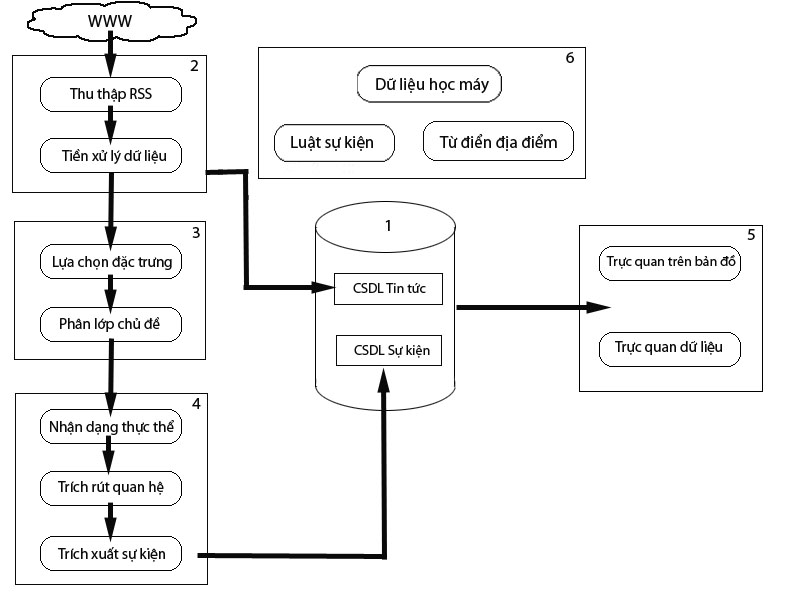
\includegraphics[width=1\textwidth]{system}
		\caption{\textbf{Mô hình hệ thống  $\mathcal{N}$\texttt{ewSOMoni}}}
		\label{fig:system}
\end{figure}




% ---------------------------------------------------------------------------
%: ----------------------- end of thesis sub-document ------------------------
% ---------------------------------------------------------------------------
